La base de datos que representa la \textbf{Figura \ref{fig: Modelo_Relacional}} es de tipo relacional, la cual debe contar las tablas y sus respectivas claves primarias, relaciones y restricciones. Este tipo de base de datos puede ser tratada como si estuviera orientada a objetos. Su diseño varía de acuerdo a los cambios que se realizan en el Modelo de Datos. 

\begin{figure}[htb]
    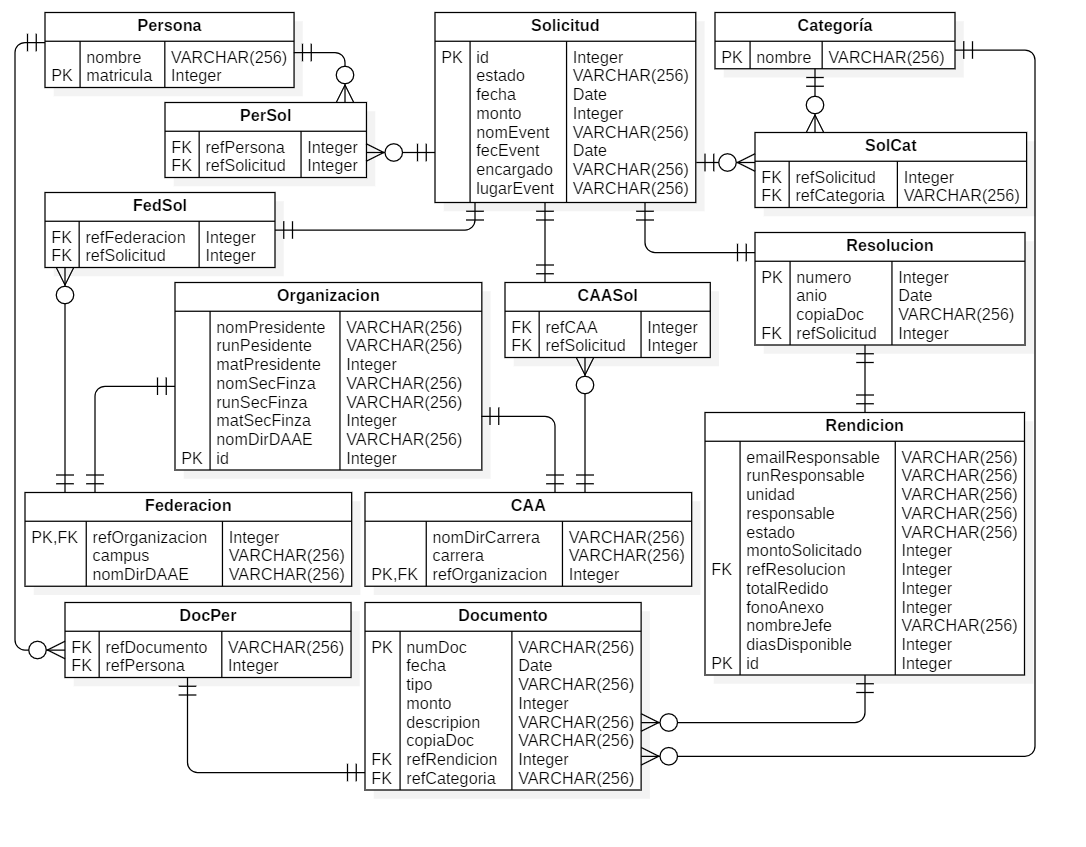
\includegraphics[width=\textwidth]{Imagenes/Modelo_relacional_bd.png}
    \caption{\label{fig: Modelo_Relacional}Modelo Relacional de la Base de Datos del sistema.}
\end{figure}

Por otra parte, se guardan cada Categoría que aparecen en el sistema para ser utilizadas en las solicitudes y especificar en que llevaron a cabo los gastos. En cuento a las listas que se realizan en el modelo de datos, se registran en la BD a través de tablas intermedias. Por último, se realizan procedimientos almacenados para el registro de los datos que provienen desde la capa de negocio. 

%Se realiza este procedimiento debido a que aumenta la rapidez de procesamiento de las peticiones del usuario ya que estas consultas se encuentran bajo el control del motor del gestor de BD.
